\documentclass{article}
\usepackage{geometry}
 \geometry{
 letterpaper,
 left=1in,
 right=1in,
 top=1in,
 bottom=1in,
 }
\usepackage[utf8]{inputenc}
\usepackage[T1]{fontenc}

\usepackage{amsmath,float}
\floatplacement{figure}{H}
\usepackage{hyperref}
\usepackage{tikz,pgfplots}
\pgfplotsset{compat=1.12}

\graphicspath{{./images/}}
%% Commande supplémentaire

% semi-norm of a vector
\newcommand{\snorm}[1]{\left| #1 \right|}
% norm of a vector
\newcommand{\norm}[1]{\left\| #1 \right\|}
% degree symbol
\newcommand{\degree}[0]{^\circ} 
% rename builtin command \v{} to \vaccent{}
\let\vaccent=\v 
% for vectors
\renewcommand{\v}[1]{\ensuremath{\mathbf{#1}}} 
% for vectors of Greek letters
\newcommand{\gv}[1]{\ensuremath{\mbox{\boldmath$ #1 $}}} 
% for unit vector
\newcommand{\uv}[1]{\ensuremath{\mathbf{\hat{#1}}}}	
% for tensors
%\newcommand{\tn}[1]{\ensuremath{\pmb{\mathsf{#1}}}} 
% for tensors of Greek letters
\newcommand{\tn}[1]{\ensuremath{\mbox{\boldmath$\mathsf{#1}$}}} 
% for absolute value
\newcommand{\abs}[1]{\left| #1 \right|}	
% for average
\newcommand{\avg}[1]{\left< #1 \right>} 
% rename builtin command \d{} to \underdot{}
\let\underdot=\d 
% for derivatives
\renewcommand{\d}[2]{\frac{d #1}{d #2}} 
% for double derivatives
\newcommand{\dd}[2]{\frac{d^2 #1}{d #2^2}} 
% for partial derivatives
\newcommand{\pd}[2]{\frac{\partial #1}{\partial #2}}
% for double partial derivatives
\newcommand{\pdd}[2]{\frac{\partial^2 #1}{\partial #2^2}} 
% for crossed double partial derivatives
\newcommand{\pdx}[3]{\frac{\partial^2 #1}{\partial #2 \partial #3}} 
% for thermodynamic partial derivatives
\newcommand{\pdc}[3]{\left( \frac{\partial #1}{\partial #2} \right)_{#3}} 
% for Dirac bras
\newcommand{\ket}[1]{\left| #1 \right>} 
% for Dirac kets
\newcommand{\bra}[1]{\left< #1 \right|} 
% for Dirac brackets
\newcommand{\braket}[2]{\left< #1 \vphantom{#2} \right| \left. #2 \vphantom{#1} \right>} 
% for Dirac matrix elements
\newcommand{\matrixel}[3]{\left< #1 \vphantom{#2#3} \right| #2 \left| #3 \vphantom{#1#2} \right>} 
% for gradient
\newcommand{\grad}[1]{\gv{\nabla} #1}
% rename builtin command \div to \divsymb
\let\divsymb=\div 
% for divergence
\renewcommand{\div}[1]{\gv{\nabla} \cdot #1} 
% for curl
\newcommand{\curl}[1]{\gv{\nabla} \times #1} 
% for laplacian
\newcommand{\lap}[1]{\gv{\nabla}^2 #1}
% Math text
\newcommand{\mt}[1]{\mathrm{#1}} 
% Overline
\newcommand{\ol}[1]{\overline{#1}}
% Partial derivative with dfrac
\newcommand{\dpd}[2]{\dfrac{\partial #1}{\partial #2}}
% Scientific notation
\providecommand{\e}[1]{\ensuremath{\times 10^{#1}}}
% Symbole degré
\renewcommand{\deg}{$^{\circ}\;$}

% text style
%
\newcommand{\Ae}{\text{\normalshape a.e.}}
% c'est-à-dire
\newcommand{\ie}{\textit{i.e.}\ }
% e.g. - par exemple
\newcommand{\eg}{\textit{e.g.}\ }
\newcommand{\strong}{\text{\normalshape -strong}}
\newcommand{\weak}{\text{\normalshape -weak}}
\newcommand{\loc}{\text{\normalshape loc}}
\newcommand{\ad}{\text{\normalshape ad}}
% Symbole degré
\renewcommand{\deg}{$^{\circ}\;$}
% Accronymes
\newcommand{\PIV}{\textit{PIV}\ }

% Space operator
\newcommand{\Def}{\overset{\text{\textup{def}}}{=}}
\newcommand{\R}{\operatorname{\mathbb R}}
\newcommand{\Rn}{\operatorname{{\mathbb R}^N}}
\newcommand{\RK}{\operatorname{{\mathbb R}^K}}
\newcommand{\N}{\operatorname{\mathbb N}}
\newcommand{\Z}{\operatorname{\mathbb Z}}
\newcommand{\ON}{\operatorname{\text{\textup{O(N)}}}}
\newcommand{\opt}{\mathrm{opt}}

% Matrix operator
\newcommand{\transp}{\:{}^*\,\negmedspace}
\newcommand{\trans}{\:{}^* \negmedspace}
\newcommand{\transm}{\:{}^* \!\negmedspace}
\newcommand{\tran}{{}^* \negmedspace}

% Environnement pour les Théorème, lemmes et remarques
\newtheorem{theoreme}{Th\'{e}or\`{e}me}
\newtheorem{lemme}{Lemme}
\newtheorem{remarque}{Remarque}
\newtheorem{prop}{Proposition}
\newtheorem{hypo}{Hypoth\`{e}se}
\newtheorem{dfn}{D\'{e}finition}

% Variables
\newcommand{\constant}[1]{\mathit{#1}}
\renewcommand\Re{\constant{Re}}  % Reynolds number
\newcommand\Pe{\constant{Pe}}  % Peclet number
\newcommand\Nu{\constant{Nu}}  % Nusselt number
\newcommand\Sh{\constant{Sh}}  % Sherwood number
\newcommand\Sc{\constant{Sc}}  % Schmidt number
\renewcommand\Pr{\constant{Pr}}  % Prandlt number
% Trucs de chimie
\newcommand\el{\mathrm{e^-}}
\newcommand*\chem[1]{\ensuremath{\mathrm{#1}}}

% used tikz libraries
\usetikzlibrary{patterns}
\usetikzlibrary{arrows}
\usetikzlibrary{calc}
\usetikzlibrary{intersections}
\usetikzlibrary{trees}
\usetikzlibrary{positioning}
\usetikzlibrary{arrows}
\usetikzlibrary{chains}
\usetikzlibrary{decorations.shapes}
\usetikzlibrary{decorations.pathreplacing}
\usetikzlibrary{decorations.pathmorphing}
\usetikzlibrary{decorations.markings}
\usetikzlibrary{shapes}
\usetikzlibrary{matrix}

\begin{document}

\begin{figure}[!ht]
\centering
\begin{tikzpicture}
    \begin{axis}[
        width=13cm,
        height=8cm,
        xlabel=\textsc{Wow such x axis},
        ylabel=More y
    ]
      \addplot plot [smooth] file {data/lcs_neg_graph.dat};
      \addplot plot [smooth] file {data/lcs_pos_graph.dat};
      \legend{Line A\\Line B\\}
   \end{axis}
\end{tikzpicture}
\caption{Simple example using pfgplots axis}
\end{figure}

\begin{figure}[!ht]
\centering
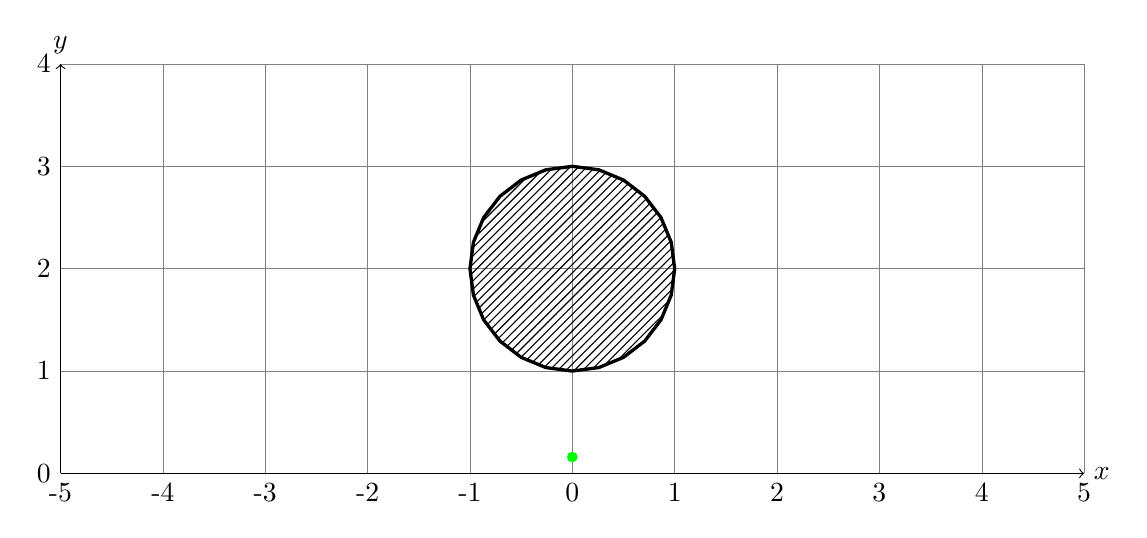
\begin{tikzpicture}[scale=1.3]

 % size
  \def\xmin{-5}
  \def\xmax{5}
  \def\ymin{0}
  \def\ymax{4}

  % grid
  \draw[style=help lines, ystep=1, xstep=1] (\xmin,\ymin) grid (\xmax,\ymax);

  % axes
  \draw[->] (\xmin,\ymin) -- (\xmax,\ymin) node[right] {$x$};
  \draw[->] (\xmin,\ymin) -- (\xmin,\ymax) node[above] {$y$};

  % xticks and yticks
  \foreach \x in {\xmin,...,\xmax}
      \node at (\x, \ymin) [below] {\x};
  \foreach \y in {\ymin,...,\ymax}
      \node at (\xmin,\y) [left] {\y};
  
% circle  
  \draw[domain=0:360, very thick, pattern = north east lines] plot ({cos(\x)}, {sin(\x)+2});
  \fill[color=green] (0,0.16) circle (1.5pt);
  
  % 2 lines
  \draw[color=blue] plot [smooth] file {data/lcs_neg_graph.dat};
  \draw[color=red] plot [smooth] file {data/lcs_pos_graph.dat};
\end{tikzpicture}
\caption{This is using tikz instead of pgfplot and drawing everything by hand.}
\end{figure}


%=== RÉSULTATS MÉTHODE INVERSE 2D ===%
\begin{figure}[!ht]
\centering
\begin{tikzpicture}
\def\chemin{data/2D_f5000_beta05_new.txt}
\begin{axis}[
width=11cm,
height=8cm,
xmin=0, xmax=1.5,
%ymin=0,        
ylabel=\textsc{$S^*$},
xlabel=\textsc{$t^*$},
ylabel style={rotate=-90},
legend style={font=\tiny},
title={$f^*=5000$}
]

\addplot+[no marks]
table[x index=0,y index=1] {\chemin};
\addplot+[no marks, dashdotted]
table[x index=0,y index=2] {\chemin};
\addplot+[mark size=1.5pt, mark=x]
table[x index=0,y index=3] {\chemin};
\addplot+[only marks, mark size=1.2pt, mark=o]
table[x index=0,y index=4] {\chemin};
\legend{$S_{exp}$ \\ $S_q$ \\ $S_{sob}$ \\ $S_{inv}$ \\}

\end{axis}
\draw (9.8,0) node{};
\end{tikzpicture}
\caption{Plot data from different collumn in the same data file}
\end{figure}

\begin{figure}[!ht]
\centering
\begin{tikzpicture}

% plot curve for first axis
\begin{axis}[
width=11cm,
height=8cm,
xmin=0, xmax=1,
ylabel={$u_1$ [m/s]},
xlabel={$t^*$},
axis y line=left,
legend style={draw=none}
]
\addplot[mark=o] table[x index=0,y index=1] {data/moy_phase_4hz.dat};

% add label to access plot from first axis
\label{plot_one};
\end{axis}

% plot curves for second axis
\begin{axis}[
width=11cm,
height=8cm,
xmin=0, xmax=1,
ylabel={$u_2$ [m/s]},
xlabel={$t^*$},
axis y line=right,
ylabel style={yshift=-0.5em},
axis x line=none
]

% add the item of the first axis referencing axis !!
\addlegendimage{/pgfplots/refstyle=plot_one}\addlegendentry{$u_1$: Piston, 4~Hz}

% then we use add plot for curves on second axis
\addplot[color=red,mark=x] table[x index=0,y index=1] {data/moy_phase_34hz.dat};
\addplot[domain=0:1,dashed,thick]{0.030759*sin(deg(2*pi*x)-7)+0.730899065};

% that we also create legend entry
\addlegendentry{$u_2$: P.-à-f., 34~Hz}
\addlegendentry{Fonction sinus}
\end{axis}
\end{tikzpicture}
\caption{Two axis from different file using one combined legend}
\end{figure}


%=== ÉCOULEMENT PULSÉ CANAL ===%
\begin{figure}[!ht]
\centering
\begin{tikzpicture}
\def\chemin{data/poiseuille_pulse2.txt}
\def\file{data/poiseuille_pulse_theo2.txt}

\begin{axis}[
width=10cm,
height=8cm,
xmin=0, xmax=1,
ylabel={$u~$[m/s]},
xlabel={$t^*$},
mark size=1.5pt,
legend style={font=\footnotesize}
]
\addplot+[only marks,mark=o]
table[x index=0,y index=1] {\chemin};
\pgfplotsset{cycle list shift=-1}
\addplot+[no marks, dashed]
table[x index=0,y index=1] {\file};
\addplot+[only marks,mark=o]
table[x index=0,y index=2] {\chemin};
\pgfplotsset{cycle list shift=-2}
\addplot+[no marks, dashed]
table[x index=0,y index=2] {\file};
\addplot+[only marks,mark=o]
table[x index=0,y index=3] {\chemin};
\pgfplotsset{cycle list shift=-3}
\addplot+[no marks, dashed]
table[x index=0,y index=3] {\file};
\legend{$z_0$, exp. \\ $z_0$, ana. \\ $z_1$, exp. \\ $z_1$, ana. \\ $z_2$, exp. \\ $z_2$, ana. \\}
\end{axis}

% Canal
% Plancher
\foreach \x in {7,6.7,...,4}{
	\draw[thick] (\x+5,2) -- (\x-0.25+5,2-0.25);
	\draw[thick] (\x+5,5.25) -- (\x-0.25+5,5.25-0.25);
}
\draw[thick] (12,2) -- (9,2);
\draw[thick] (12,5) -- (9,5);

% Axes
\draw (10.71,3.52) node {$\bigotimes$} node[below right]{\small$x$};
\draw[->,thick,>=latex] (10.53,3.52) -- +(-1.2,0) node[below] {\small $y$}; 
\draw[->,thick,>=latex] (10.7,3.67) -- +(0,1.2) node[right] {\small$z$};

% Points et hauteur
\draw[<->] (11.8,2) -- node[left] {\footnotesize$h$} (11.8,5);
\fill[blue] (10.1,3.51) node[above left] {\scriptsize $z_0$} circle (2pt);
\fill[red] (10.1,3.91) node[above left] {\scriptsize $z_1$} circle (2pt);
\fill[brown] (10.1,4.6) node[above left] {\scriptsize $z_2$} circle (2pt);

%Notes
\draw (10.2,1.3) node(x){\footnotesize $x\equiv$ direction de};
\draw ($(x)+(0.4,-0.35)$) node{\footnotesize l'écoulement};
\draw ($(x)+(-0.3,-1)$) node{\footnotesize $h\simeq3.3$~mm};
\draw (12.5,0) node{};
\end{tikzpicture}
\caption{Curves with geometry on the side}
\end{figure}

\begin{figure}[!ht]
\centering
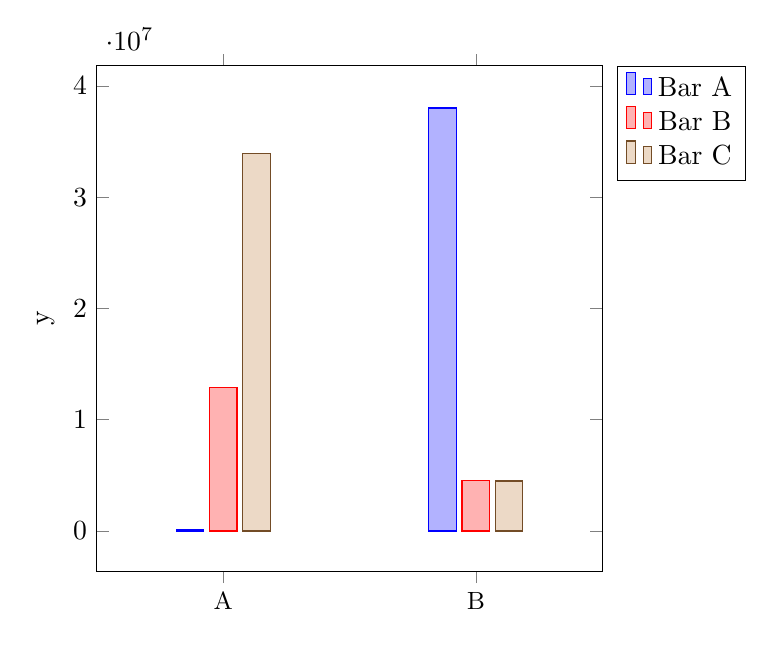
\begin{tikzpicture}
\begin{axis}[
    width=8cm,
    height=8cm,
    ylabel=y,
    legend style={legend columns=1}, 
    legend pos=outer north east,
    ybar,
    bar width=10pt, 
    symbolic x coords={A, B},
    x tick label style={font=\small,text width=1.7cm,align=center},
    xtick=data,
    enlarge x limits=.5]

\addplot coordinates {(A,166598) (B,38006949)};
        
\addplot coordinates {(A,12920610) (B,4538630)};
          
\addplot coordinates {(A,33958673) (B,4500302)};

\legend{Bar A,Bar B, Bar C}
\end{axis}
\end{tikzpicture}
\caption{Simple histogram plot}
\label{fig:histogram}
\end{figure}

\end{document}